\documentclass[11pt]{article}
\usepackage{acl2015}
\usepackage{times}
\usepackage{url}
\usepackage{latexsym}
\usepackage{epsfig}
\usepackage{amsmath}

\begin{document}



%title{Modeling for Query Linguistic Analysis System (QLAS)}
%\author{Ruiqiang Zhang Yi Chang\\
%Yahoo! Inc \\
%701 First Avenue, Sunnyvale, CA94089 }
%\date{}




\title{Diversified Named Entity Recognition for Web Search Query}

\author{Ruiqiang Zhang \\
%  Affiliation / Address line 1 \\
%  Affiliation / Address line 2 \\
%  Affiliation / Address line 3 \\
%  {\tt email@domain} \\\And
  \And   Youssef Billawa \\
%  Affiliation / Address line 1 \\
%  Affiliation / Address line 2 \\
%  Affiliation / Address line 3 \\
%  {\tt email@domain} \\}
 \And Yi Chang 
%\\}
}
\maketitle


\begin{abstract}
This paper propose using  gradient boosted decision tree (GBDT) method in natural language processiong to attack named entity recognition (NER) on Web search query task,. This approach performs significant different results comparing to the well-known CRF method. While the CRF produces the best top 1 NER, we found the CRF was inferior to the GBDT in dealing with ambiguous queries with multiple intents.  Due to query intent ambigurity, the CRF-based NER generates less diversified results and has lower precision for queries with multiple intents. The proposed GBDT method can achieve better diversity results because of global features, subjective judgement as training targets and multiple sources to generate named entities. Our experiments prove the GBDT signifiantly improved NER accuracy.
\end{abstract}





\section{Introduction}

Query is ambiguous. Web search users usually send short and ambiguous queries because they want to get fast search results. Search engines have to adapt to such incomplete queries to guess search intents. "Apple" can mean different things by user. It could be a fruit (Food), or apple product (Brand) or apple corporate (Business). Discovering query intent is an important factor for improving Web search user experience. All the ambiguous query intents should be detected by search engines.  A good search engine can give diversified search results. She can understand and translate  queries into multiple categories. Top search engines such as Google, Bing and Yahoo can present users with results from different categories. Some typical categories include Product, Shopping, Travel, Local, etc.  These category search results are positioned on the eye-striking places  on the  on search result page. They are called Direct Display (DD) by some search engines.   DD Search retrieves content from storages of a specific category. Therefore, given their important layout, understanding query intent is critical in these tasks. 

%% If a query has shopping intent, Category Search shows search results from shopping listings.
\begin{table*}
\begin{center}
\begin{tabular}{|c|l|c|} \hline
 & interpretation & subjective judgement \\ \hline
1 & [napa]\_Place  [auto repair]\_Business & Excellent \\ \hline
2 & [napa]\_Place  [auto]\_Business    [repair]\_token & Good \\ \hline 
3 & [napa]\_Place  [auto]\_token  [repair]\_token & Fair \\ \hline
4 & [napa auto repair]\_Organization & Excellent \\ \hline
5 & [napa]\_Organization  [auto repair]\_Business &  Excellent \\ \hline
\end{tabular}
\caption{An example of ambiguous query interpretation. Last column is subjective judgement.}
\end{center}
\label{table:diversity}
\end{table*}



NER is one of the big techniques in query intent understanding. Most published work on NER is related to text-based. But  query NER is quite different from text. The task difficulty of query NER is higher than that of text NER. This can be seen from calculating language model's perplexity. Perplexity of trigram language model in our work on Web search queries is 385, while the value is 141 for normal English text (evaluated by WSJ treebank~\cite{Mikolov:2012}).  Higher perplexity is because query is ambiguous, non-grammatical, and less  contextual information available. These are reasons why query NER have lower accuracy than text NER. Diversity is a new problem for query NER. There are many cases that  queries have multiple intents. All entity types have to be generated. Otherwise, search results may be biased to one intent and lose other intents.   This requirement has not been considered in the existing text-based NER. Traditional NER only considers generating the best entity type. This is weakness of all existing methods including the CRF.
 
The most widely used NER method is CRF which has  the state-of-the-art performance in text-based NER, as reported~\cite{McCallum:2003:ERN:1119176.1119206}. The open source NER toolkit developed by Stanford University uses CRF as the main algorithm~\footnote{http://nlp.stanford.edu/software/CRF-NER.shtml}.  However,  we find that the CRF is not a good method for dealing with  query intent ambigurity.  Even if CRF generates multiple (top 3) results, those results can be very similar. It is because the CRF scoring method is based on the whole query entities which can be approximated as the  sum of every entities' score. The whole query score is very likely to be dominated by a single token. That is, the global score is controlled by a strong local maximum.   Due to this, multiple output can have very similar results. Diversity is an inherent problem for the CRF. We will further explain this in section~\ref{sec:crf}.
 An example is shown in Table~\ref{table:diversity}. For the query ``napa auto repair", ``napa"'s meaning is ambiguous. It could be a city name or a business name.  Table~\ref{table:diversity} lists five interpretations from the CRF.  To simpify, we use ``interpretation" to mean one result of whole entity tagging on the query. All of the top three interpretations tag "napa" as Place because it is a dominated entity. The last two labels ``napa" as Organization. But the last two can probably be missed if only top three are used. 

In light of CRF's diversity problem on query NER, this work adopts a decision tree based method on the ground of the CRF based results. In this framework, the CRF plays the role as one of query interpretation generation methods, together with other two methods: dictionary based and rule-based. All three methods each generates a few candidate interpretations and then the process is followed by a decision tree based re-ranking. We used gradient boosted decision tree (GBDT)\cite{Friedman:2002,Ye:2009}  model. We found this model could reduce diversity problem by two reasons: one is global features and using editorial subjective judgement as training target. We give the details in section~\ref{sec:gbdt}.










%%89.31%


\section{Related Work}
NER has been a long time research area in natural language processing. Traditional NER target is text-based  named entity. All sort of machine learning methods have been applied this field and  there are many publications. Traditionally, methods can be classified as unsupervised~\cite{Collins:1999,Etzioni:2005:UNE:1090483.1090487}, semi-supervised~\cite{Riloff:1999:LDI:315149.315364,Ji:2006:DSS:1641408.1641414} and supervised according to whether human labelled data is used in training. It can be support vector machine~\cite{Asahara:2003:JNE:1073445.1073447}, hidden markov model~\cite{Shen:NER}, maximum entropy~\cite{Chieu:2003:NER:1119176.1119199}, conditional random fields~\cite{McCallum:2003:ERN:1119176.1119206}  according to algorithm. The best NER result evaluated in the CoNLL  conferenece~\cite{TjongKimSang:2003:ICS:1119176.1119195} using NER shared-task data is 88.76\% in terms of F1, where the authors used a multiple classifier combining method linear,HMM, transform based learning (TBL), and ME. 
Recently, deep learning method is found to achieve state-of-the-art results, 89.59\%, on the same data~\cite{collobert:2011b} .

CRF is widely used in many NLP tasks including word segmentation~\cite{Xue:2003:CWS:1119250.1119278}, parsing~\cite{Sha:2003:SPC:1073445.1073473} and named entity recoginition~\cite{McCallum:2003:ERN:1119176.1119206}. In all these fields, CRF was found higher accuracy than the existing methods such as SVM, HMM and ME.

There are many existing work in text-related NER as mentioned above. Less literatures have been found for query NER. Actually, query NER is very important for search because 85\% of web search queries contains one or more entities~\cite{Lin:2012}. The work of \cite{Lin:2012,Pantel:2012:MET:2390524.2390603}  describes their approach to find query intent where EM algorithm is applied on large query set and using url-click information. In their work, 73 entity type is defined and 147K entities are extracted from Freesbase. Their work limits only one single entity inside a query. 

There are some work on query segmentation. The task is to divide query into multiple segments correctly based on entity but not need to label entity type.
\cite{Hagen:2012} described an overview of state-of-the-art work in query segmentation.  The best word segmentation results are around 85\%. 

The paper \cite{Guo:2009:NER} proposes a probabilistic approach to the named entity recognition using query log data and Latent Dirichlet Allocation. Topic model is constructed by a weakly supervised LDA method. The method is tested on a tag set with only 4 taxonomies related to media. The best NER accuracy as reported is 80\% on the four categories. However, the evaluation was based on known query segmentation. The results will be worse if segmentation is not known as in our work.



Decision tree (DT) method was used in the early stage of NLP~\cite{Black:1993,Magerman95statisticaldecision-tree}. This approach was replaced by more advanced models such as maximum entropy and CRF. The old DT is a classification model that mixmizes classification error rate.  Our DT model is based on the work of \cite{Friedman:2002,Ye:2009}, gradient boost decision tree (GBDT). The DT in our work is a regression model that optimizes editorial grades. The model has been widely applied into many machine learning tasks, for example, Web search ranking~\cite{Ye:2009}. 


\section{Non-diversity of the CRF tagging model}
\label{sec:crf}

\begin{figure*}
\centering
\epsfig{file=crflocal2.png, height=2in, width=4in}
\caption{CRF local maximum: $y_{21},y_{22},y_{23}$ are word $x_{2}$'s candidates tags. $y_{21}$ is a local maximum tag. All top tag sequences have to pass it other than two other tags.$y_{21}$ suppresses $y_{22}$ and $y_{23}$ in ambiguous query tagging.}
\label{fig:crflocal}
\end{figure*}

We used three approach methods to generate query interpretation candidates: maximum length match (MLM), heuristic rule based (HRB), and CRF tagging. CRF tagging is the most effective method. But MLM and HRB can provide additional candidates. Our NER system has a knowledge repository that stores millions of entities. Query interpretation by the MLM is through entity match with the entites in the knowledge base. Use the longest query words from left to right to match entites until a match is found. Continue to match anther longest entity starting from the unmatched position of the query. Continue the process until all query words are gone through.  This is a greedy search from left to right.  MLM is able to generate candidates such as No.1, No.4 and No.5 of Table~\ref{table:diversity} because it is either full match of an entity or partial match by two entities. 

HRB is based on rules. We have created rule base consisting of hundreds of patterns. Each pattern defines a full parse consisting of words and entities. And a score is given for each rule. The score is proportional to frequency of the rule occurring in the query log.  For example, No.1 of Table~\ref{table:diversity} can be generated by ``Place + Business" pattern. 

The CRF is undirected graphical model~\cite{lafferty:2001}.  The CRF tagging illustration is shown in Fig.~\ref{fig:crflocal}. The figure shows a six-word query. The query sequence is $X={x_0,x_1,\cdots,x_N}$. The labels are $Y={y_0,y_1,\cdots,y_N}$.  $y_i$ is $x_i$'s tag. $y_{i}$ is one tag of a candidate tag set. Figure~\ref{fig:crflocal} shows three  candidate tags for each word.  These candidates are decided by the
CRF tagging model that calculates  the joint probability of the entire sequence of labels as the  following formula,

\begin{equation}
p(Y|X)=\frac{1}{Z(X)}\prod_{t=1}^{T}exp{\sum_{k=1}^{K}\theta_{k}f_{k}(y_{t},y_{t-1},x_{t})}
\label{eq:crf}
\end{equation}

$f_{k}(y_{t},y_{t-1},x_{t})$ is features. $\theta_{k}$ is model's parameters, which are estimated by maximizing log likelihood of training data.

Which path has the highest value of~\label{eq:crf} will be  the top 1 resulting tag sequence. Fig.~\ref{fig:crflocal} also illustrates local maximum problem. If $p(y_2)=y_{21}|X)\gg p(y_2\neq y_{21}|X)$, all tag sequences will pass through $y_{21}$. As results, $y_{22}$ and $y_{23}$ are unlikely to be chosen. There are multiple reasons to have local maximum. \textit{Label bias} in training is one cause. Training data may  be biased to one entity over others. Like query ``apple tree". If majority of ``apple" in training has ``Organization" entity type, it is unlikely to recogize ``apple tree" as ``Fruit". The label bias  is very easy to happen for query NER because the entities are huge and diversified.  \textit{Label bias} issue was raised in~\cite{lafferty:2001}. While the CRF is a theoratical solution to attack label bias problem~\cite{lafferty:2001}, we observed a large amout of  local maximum for query NER problem. There are other reasons to cause local maximum like local features.   
CRF uses many local features instead of global features. Either global features are not easy to implement or it is not efficient in the CRF method. Local features may cause the local maximum. On the contrary, GBDT use  a lot of global features.    


%%$$
%%\sum_{i=1}^{N}\sum_{t=1}^{T}\sum_{k=1}^{K}\theta_{k}f_{k}(y_{t}^{(i)},y_{t-1}^{(i)},x_{t}^{(i)})-\sum_{i=1}^{N}logZ(x^{(i)})
%%$$ 

We adopted the common methods, ``BIO" tagging, for NER tagging using the CRF~\cite{Xue:2003:CWS:1119250.1119278}. ``B" and ``I" specify an entity boundary, either the beginning or intemediate position of an entity. ``O" indicates non-entity word.  This method can map a query word sequence to an entity sequence throught one-by-one alignment.
For example, ``tom cruise movie" maps to ``B\_Person I\_Person O". This mapping method is a typical use of  the CRF tagging method.
Named entities can be easily obtained by simply mapping the BIO sequence to entity sequence. Both entity and entity boundary are extracted.  

This work used many new features that is unique for query NER. Our model used about 30M features due to diversified web vocabulary and rich query context. We used the following information as features: precede/current/next query word, word position, word boundary, word spelling, lexical and query word topics. Topics were created by the latent dirichlet allocation (LDA) over 10 million queries. Our training data were selected randomly from query log and manually labeled by editors. 

In decoding stage, multiple interpretations can be produced and the order of interpretations is ranked according to the value of $p(Y|X)$. Note $p(Y|X)$ is conditional probability. The best tag sequence has the highest value holds only in condition of given $X$. $p(Y|X)$ is meaningless globally. We can't judge whether a CRF interpretation is good or not according to $p(Y|X)$. What we can only tell  is the best tag sequence  relative to other results given the tag sequence,$X$.   Using $p(Y|X)$ as a criteria to select good interpretations was disappointed.  However, GBDT can tell good interpretations from bad ones because the GBDT score is meanful globally. 


\section{GBDT rescoring model}
\label{sec:gbdt}


The re-scoring function is a logistic regression model. The probability is given by the formula below,
\begin{equation}
\begin{array}{l}
p(x) = \frac{1}{1+e^{(a*(b-f(x))}}\\ 
y=\left \{\begin{array}{cc} +1 & p(x)> threshold \\ -1 & othervise \end{array}\right.
\label{eq:gbdt}
\end{array}
\end{equation}

where $x$ is the generated feature vector for a given query and interpretation. $a$ and $b$ are the slope and pivot parameters. $a=2.0$ and $b=2.6$ are determined by optimizing classifier's performance in terms of recall and precision. $\{+1,-1\}$ denotes good interpretation and bad interpretation. $thrshld$ is set to separate good and bad interpretation according to the score $p(x)$. 

We employ Gradient Boosted Decision Tree algorithm 
to learn the function $f(x)$. Gradient Boosted Decision Tree is an
additive regression algorithm consisting of an ensemble of trees,
fitted to current residuals, gradients of the loss function, in a
forward step-wise manner. It iteratively fits an additive model as

%\begin{align}
$$
f_t(x) = T_t(x; \Theta) + \lambda \sum_{t=1}^T \beta_t T_t(x; \Theta_t)
$$
%\end{align}
\noindent such that certain loss function $L(y_i, f_T (x + i))$ is
minimized, where $T_t(x;\Theta_t)$ is a tree at iteration $t$,
weighted by parameter $\beta_t$, with a finite number of parameters,
$\Theta_t$ and $\lambda$ is the learning rate. At iteration t, tree
$T_t(x; \beta)$ is induced to fit the negative gradient by least
squares.


\noindent The optimal weights of trees $\beta_t$ are determined by
%\begin{align}
$$
\beta_t = \text{argmin} _{\beta} \sum_i^N L(y_i, f_{t-1}(x_i) + \beta T(x_i, \theta))
$$
%\end{align}


GBDT model is supervised machine learning. It needs manually created training data.
The process of creating training data is as follows. We randomly sampled hundreds of thousands of queries from Web search query log. For each query, we run CRF tagger to get top candidate interpretations. In addition, we generated more interpretations by MLM and HRB. Editors assign 4 grades EGFB (Execllent, Good, Fair, Bad), to each of (query, interpretation) pairs. We show some examples on the last column of Table \ref{table:diversity}. 
Grade `E' is assigned to an excellent interpretation where all entities are correctly spanned and tagged. This interpretation will almost definitely lead to search results that are much better than those generated by the `default interpretation' (where all words are just `token').
Grade `G' is assigned to a good interpretation where some entities but not all are correctly spanned and tagged. For example, some entities will not be tagged at all or tagged with a very general tag. This interpretation may lead to search results that are better than the default interpretation, but these could be further improved.
%This is a broad category that can range from only one tag being correct and all other tags tokens, to all tags being correct but one of them failing to go to the second %hierarchy level.
Grade `F' is the baseline grade and default level of interpretation. It is no better or worse than if each word was treated as an individual keyword match. Queries with all spans marked as ``token" are considered Fair. The exception to this rule is a query whose only interpretation are all spans labeled ``token". In this case, the interpretation is marked Good.
Grade `B' is a bad interpretation; some of the important entities are not spanned or tagged correctly, in a way that leads to a wrong understanding of the query.




\section{Features of GBDT}

Features used in the GBDT are completely different from those in the CRF. GBDT feature value can't be string. Contextual features can't be used in GBDT. All GBDT features' values are real values. Feature size is very different. We used 30M features in CRF, but only 500 in GBDT. But GBDT can use global features.  We show some global features in Table.~\ref{table:features}. Those global features are not available in CRF. Some features are very useful. For example, No.1 is number of recognized entities. It is a good feature to  distinguish "napa" as Place from as Organization. is No.3 is tag language model (LM) score for whole sentence. No.4 is count of generation methods that can generate the interpretation. Its function likes a voting strategy.   No.6 is number of entities stored in taxonomy.
\begin{table}
\begin{center}
\begin{tabular}{|c|l|}\hline
 1 & number of entities \\ \hline
 2 & number of non-recognized tokens \\ \hline
 3 & tag LM score of whole query \\ \hline
 4 & number of generation methods \\ \hline
 5 & crf model score \\ \hline
 6 & number of taxonomy match \\ \hline
\end{tabular}
\caption{GBDT global feature examples}
\label{table:features}
\end{center}
\end{table}

GBDT features are generated by the following methods.
Eight features are from query level. (1) number of terms (2) number of stop words (3) number of special characters (4) number of entities recognized for this interpretation (5) number of non-tagged terms (6) number of non-token tags (7) position of first non-token tag (8) position of last non-token tag.

Four features are from CRF tagger: (1) CRF raw probability (2) rank of CRF generated interpretation (3) ratio of current CRF interpretation to the top 1 CRF interpretation. (4) a boolean feature to indicate if interpretation is from CRF tagger.

There are two types of LM scores, context-independent tag (priors) and context dependent tag ngram LM scores. Context-independent tag scores are the average prior scores of any tags in the interpretation. Context-dependent tag sequence scores are ngram LM probability. Context-independent scores do not count token but context-dependent scores include tokens.
LM was built using editorial judgment data. 200 features are extracted by this method.

Some other features include template match. We manually wrote a lot of template-based rules to recognize query intents. These rules are from multiple domains. Take the query above as examples. (napa, Place) matches a Local template rule and (napa, Organization) matches a Auto template rule. Features from template match include number of rule match.

Other features include counts of each taxonomy and ratio of each taxonomy if the query interpretation has multiple taxonomies. The feature size of this type is equal to the tag set. 

We defined entity confidence score based on CRF results. It is called global word posterior probability in ~\cite{Soong_generalizedword}. Assume CRF generates $N$ query interpretations. Entity $e$ may or may not have appearance in a interpretation $I_{i}$. If the CRF score of the interpretation is as $P(I_{i})$, then   the confidence of entity is calcuated by the formula as, 
$$
  \text{conf}(e) = \frac{\Sigma_{i}^{N} P(I_{i})\epsilon(e,I_{i})}{\Sigma_{i}^{N} P(I_i)} 
$$

Above is confidence score of one entity. From it, we genereate full interpretation score as a new feature. It is calculated as sum of all entities' confidence score recognized in the interpretation.

\section{Experiments}

%% evaluation data: 600 queries, 4k interpretation, average interpretation/queries=6.1  


\begin{table*}
\begin{center}
\begin{tabular}{|c|c|c|c|c|c|}
\hline
    \multicolumn{2}{|c|} {}    & \multicolumn{2}{|c|} { Coarse Category} & \multicolumn{2}{|c|}{ Fine Category} \\ \cline{3-6}
    \multicolumn{2}{|c|}{}      &  Accuracy-N  &  DCG-N &   Accuracy-N & DCG-N \\ \hline
N=1 & CRF  & 0.7249& 5.3 & 0.5987  & 4.5 \\ \cline{2-6}
         & GBDT  & 0.6814 & 5.2 &  5647 & 4.1 \\ \hline
N=2 & CRF  & 0.5151 & 7.9 & 0.4187& 6.5  \\ \cline{2-6}
         & GBDT  & 0.5324 &8.1 & 0.4528 & 7.4\\ \hline
N=3 & CRF  & 0.3794 &9.2 & 0.3325  &  7.1\\ \cline{2-6}
         & GBDT  & 0.4203 & 9.5 & 0.3972  & 8.5 \\ \hline
\end{tabular}
\caption{Comparison of CRF and GBDT}
\label{table:pat1}
\end{center}
\end{table*}


We predefined an in-house taxonomy set. This set has two levels of granularity: coarse level and fine level. Coarse level has 20 entity categories and Fine level has about 200 categories. Most of the widely defined categories are included in our taxonomy set such as Local, Organization, Person, Product. There are also some new categories defined specifically for business purpose. Besides type Organization, we define Brand category to emphasize shopping intent. For instance, ``apple" is an Organization for query ``apple store", and BRAND for ``apple iphone". The differing categories makes clear to separate Local intent and Shopping intent. ``apple store" has Local intent that wants to show store location, driving direction, or store hours.  ``apple iphone" has Shopping intent that shows iphone type or price list. 

For each Coarse category, a few Fine categories are defined. As an example, we define Actor, Director, Politician for Person category. Similarly, each coase category is assoicated some fine category.

%As documented in the previous sections, our whole query understanding system has two main models, CRF tagger and Scorer. The two models use different training data. CRF %tagging model uses query perfect interpretation. GBDT model training uses 4-grade judgment. A few editors took two months to create 70k perfect interpretations and 200k %EGFB data. 

Both CRF and GBDT are supervised machine learning methods. CRF needs editors to label entity for a given query.  GBDT needs editors to judge quality grade for a given query interpretation according to 4-grade judgement guideline. We submitted 60K queries to editors and returned about 80K  perfect interpretations which are used for CRF training. We collected 200K query interpretations from output of MLM,HRB and CRF and asked editors to judge these interpretations. We took 5K interpretations from 200K as evaluation data set. These 5K interpretations contain 600 queries and the average interpretations per queries is 8.2. It has 955 Excellent grade, 1051 Good, 974 Fair and 1960 Bad. 
  

Some ambiguous queries are shown in Table~\ref{table:ambiguous queries}. The examples show ambigurity could happen possiblly in many cases such as  between Brand and Product (flash player), Business and Organization (zurich life insurance) and Media and Person (billy gilman). 

\begin{table*}
\begin{center}
\begin{tabular}{|l|l|} \hline
\it{Query} & \it{Interpretation} \\ \hline
adobe flash player &          [adobe]\_Brand  [flash player]\_Brand \\
adobe flash player   &     [adobe]\_Brand  [flash player]\_Product \\ \hline

zurich life insurance &    [zurich]\_Organization    [life insurance]\_Business \\ 
zurich life insurance   &   [zurich life insurance]\_Organization \\ \hline

cars   &  [cars]\_Media:Movie  \\ 
cars    &    [cars]\_ Product:Auto  \\ \hline

windsor hotel &   [windsor]\_Place      [hotel]\_Business   \\
windsor hotel &     [windsor hotel]\_Organization  \\ \hline

albany rv &    [albany]\_Place     [rv]\_Product \\
albany rv &         [albany rv]\_Organization  \\  \hline

billy gilman &    [billy gilman]\_Media:album \\
billy gilman  &  [billy gilman]\_Person   \\ \hline


\end{tabular}
\end{center}
\label{table:ambiguous queries}
\end{table*}

The evaluation is based on the $\text{Accuracy-N}$ and the Discounted Cumulative Gain (DCG)~\cite{NDCG2000}.
$\text{Accuracy-N}$ is calculated as ``the number of interpretations that are perfect on top N interpretations divided by the total  number of  interpretations on top N". Each query has multiple perfect interpretation.
%%$$
%%\text{Accuracy-N} = \frac{\sum_{i=1}^{N}g(i)=\text{Excellent}}{\sum_}
%%$$


The DCG is computed as follows:
\begin{equation}
\nonumber
\text{DCG-N} = \sum_{i=1}^{N} \frac{g(i)}{log(1+i)}
\end{equation}
where $g(i)$ is the gain associated with the rating of result at rank $i$ and $N$ is the maximum depth result to consider.  In this paper, we use gains of $7, 3, 0.5, 0,$  respectively, corresponding to the four ratings or relevance grades.





Table~\ref{table:pat1} shows the comparison between CRF tagger and GBDT. Both coarse level and fine level results are presented. We list top 3 results.
We observed the CRF tagger is better than GBDT if top 1 interpretation is considered. But, in case of more than one interpretations, GBDT is much better than CRF.  The reasons to have improved multiple interpretations are three folds: global features, subjective training targets and using MLM and HRB to increase CRF candidates. MLM and HRB provides more diversified interpretations. Actually, accuracy of MLM and HLB are much lower than CRF. On the same evaluation set, MLM's Accuracy-1 is 0.40 and HRB's Accuracy-1 is 0.53. Both have much lower accuracy than CRF, 0.72. Even though, GBDT can take all the three methods' benefits.  

The second test to compare CRF tagger and Scorer is to evaluate precision and recall of good interpretations. The test set is (query, interpretation) pairs evaluated with EGFB grades. The CRF tagger and GBDT assign scores to each (query, interpretation) pair. A threshold can be set to determine the boundary of good and bad interpretation according to the score. Precision is calculated by the number of correctly detected E and G interpretations divided by the total number of recognized E/G interpretations. Recall is calculated by the number of correctly detected E and G interpretations divided by the total number of E and G interpretations of answers. The precision recall graph is shown in Fig.~\ref{fig:precision}. Each point is the precision and recall values corresponding to a threshold. The top green curve is of GBDT and the bottom blue curve is CRF tagger. We see Scorer is much better than CRF tagger in terms of both precision and recall.


\begin{figure}
\centering
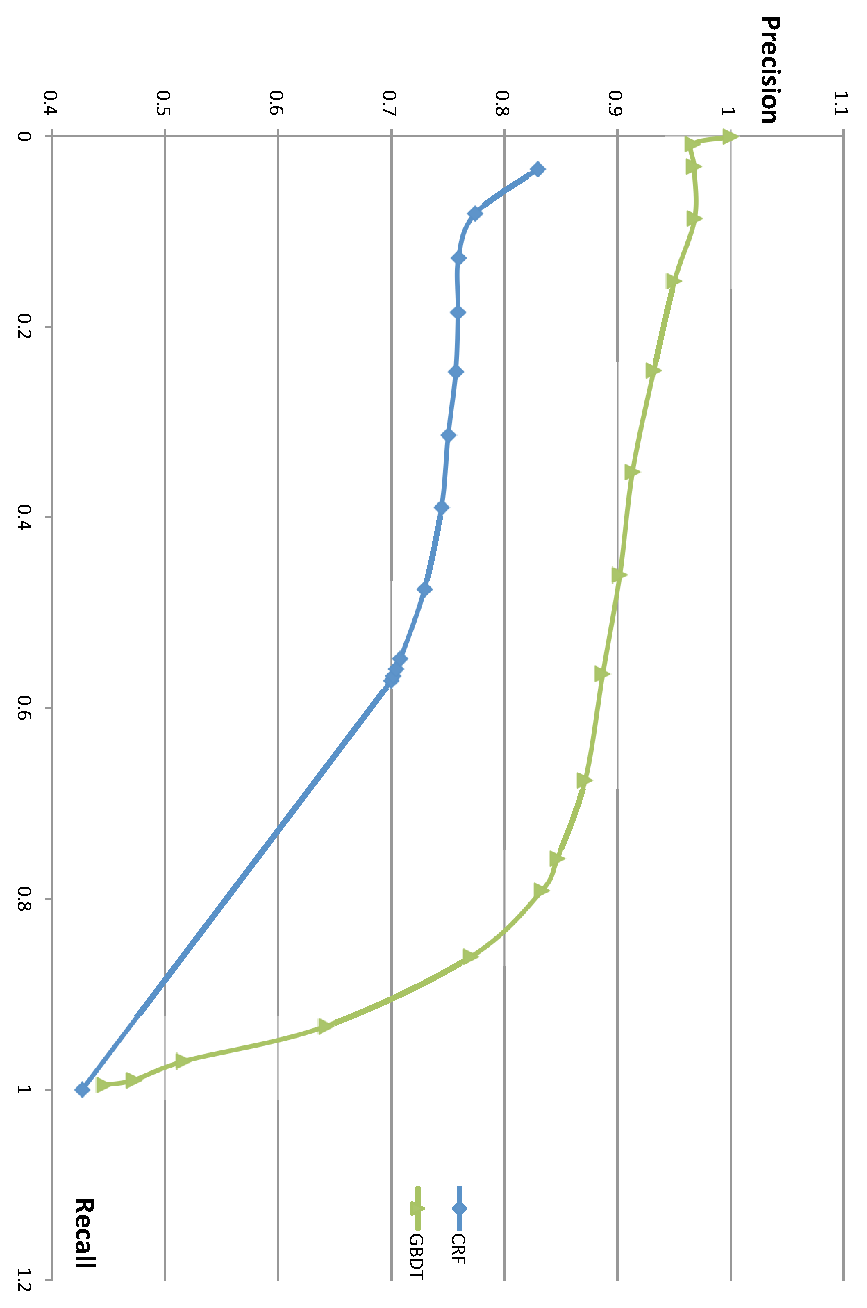
\epsfig{file=crf-gbdt-precision-recall.eps, height=3in, width=2in, angle=90}
\caption{Comparison of CRF and GBDT}
\label{fig:precision}
\end{figure}

 



\section{Conclusions}
Web query NER poses more challenge than text NER because the query is ambiguous and short of contextual information to disambigurate. Therefore, diversified results become  new problems for query NER. Our work find the flaw of the common CRF based NER when it is applied to query NER. We prove the CRF NER can't be solely used because of its local maximum, non-diversity, low precisions, and high false positive.    This work proposed a rescoring GBDT approach to fix the CRF's problem. Diversity problems are significantly reduced by applying multiple approaches: global features, global subjective judgement and addition of MLM and HRB with the CRF candidates. Our experiments prove this new framework can achieve our goals. Both precision and DCGs are improved over the CRF method. Acturally, The CRF and GBDT function differently. The CRF tagger can generate the most likely interpretations because it optimizes the likelihood of the training data.   GBDT is a regression model that maximizes subjective judgements. It can make better judgement in classifying good and bad interpretations. This is exactly what query NER wants.



\bibliographystyle{acl}

\bibliography{ner}

\end{document}




